% Preamble templated from Dhawal24112006/EE1030
\documentclass{beamer}
\mode<presentation>
\usepackage{amsmath}
\usepackage{amssymb}
%\usepackage{advdate}
\usepackage{adjustbox}
\usepackage{subcaption}
\usepackage{enumitem}
\usepackage{multicol}
\usepackage{mathtools}
\usepackage{listings}
\usepackage{url}
\def\UrlBreaks{\do\/\do-}
\usetheme{Boadilla}
\usecolortheme{lily}
\setbeamertemplate{footline}
{
  \leavevmode%
  \hbox{%
  \begin{beamercolorbox}[wd=\paperwidth,ht=2.25ex,dp=1ex,right]{author in head/foot}%
    \insertframenumber{} / \inserttotalframenumber\hspace*{2ex}
  \end{beamercolorbox}}%
  \vskip0pt%
}
\setbeamertemplate{navigation symbols}{}

\providecommand{\nCr}[2]{\,^{#1}C_{#2}} % nCr
\providecommand{\nPr}[2]{\,^{#1}P_{#2}} % nPr
\providecommand{\mbf}{\mathbf}
\providecommand{\pr}[1]{\ensuremath{\Pr\left(#1\right)}}
\providecommand{\qfunc}[1]{\ensuremath{Q\left(#1\right)}}
\providecommand{\sbrak}[1]{\ensuremath{{}\left[#1\right]}}
\providecommand{\lsbrak}[1]{\ensuremath{{}\left[#1\right.}}
\providecommand{\rsbrak}[1]{\ensuremath{{}\left.#1\right]}}
\providecommand{\brak}[1]{\ensuremath{\left(#1\right)}}
\providecommand{\lbrak}[1]{\ensuremath{\left(#1\right.}}
\providecommand{\rbrak}[1]{\ensuremath{\left.#1\right)}}
\providecommand{\cbrak}[1]{\ensuremath{\left\{#1\right\}}}
\providecommand{\lcbrak}[1]{\ensuremath{\left\{#1\right.}}
\providecommand{\rcbrak}[1]{\ensuremath{\left.#1\right\}}}
\theoremstyle{remark}
\newtheorem{rem}{Remark}
\newcommand{\sgn}{\mathop{\mathrm{sgn}}}
\providecommand{\abs}[1]{\left\vert#1\right\vert}
\providecommand{\res}[1]{\Res\displaylimits_{#1}}
\providecommand{\norm}[1]{\lVert#1\rVert}
\providecommand{\mtx}[1]{\mathbf{#1}}
\providecommand{\mean}[1]{E\left[ #1 \right]}
\providecommand{\fourier}{\overset{\mathcal{F}}{ \rightleftharpoons}}
%\providecommand{\hilbert}{\overset{\mathcal{H}}{ \rightleftharpoons}}
\providecommand{\system}{\overset{\mathcal{H}}{ \longleftrightarrow}}
	%\newcommand{\solution}[2]{\textbf{Solution:}{#1}}
%\newcommand{\solution}{\noindent \textbf{Solution: }}
\providecommand{\dec}[2]{\ensuremath{\overset{#1}{\underset{#2}{\gtrless}}}}
\newcommand{\myvec}[1]{\ensuremath{\begin{pmatrix}#1\end{pmatrix}}}
\let\vec\mathbf

\lstset{
%language=C,
frame=single,
breaklines=true,
columns=fullflexible,
showstringspaces=false
}

\numberwithin{equation}{section}

\title{MATGEO Presentation: 2.5.18}
\author{Subhodeep Chakraborty \\ ee25btech11055,\\IIT Hyderabad.}

\date{\today}
\begin{document}

\begin{frame}
\titlepage
\end{frame}

\section*{Outline}
\begin{frame}
\tableofcontents
\end{frame}

\section{Problem}
\begin{frame}
\frametitle{Problem Statement}

Let $\vec{a} = \hat{\imath} + 2\hat{\jmath} -3\hat{k}$ and $\vec{b} = 3\hat{\imath} - \hat{\jmath} + 2\hat{k}$. Show that the vectors $\vec{a}+\vec{b}$ and $\vec{a}-\vec{b}$ are perpendicular to each other.

\end{frame}

\section{Solution}
\begin{frame}{Given data}
Given vectors:
\begin{align}
 \vec{a} &= \myvec{1 \\ 2 \\ -3} \\
 \vec{b} &= \myvec{3 \\ -1 \\ 2}
\end{align}
\end{frame}

\begin{frame}{Formulae}
$\therefore$ We have:
\begin{align}
\vec{C} &= \myvec{\vec{a} & \vec{b}}\myvec{1 \\ 1} \\ %&= \myvec{4 \\ 1 \\ -1} \\
\vec{D} &= \myvec{\vec{a} & \vec{b}}\myvec{1 \\ -1} %&= \myvec{-2 \\ 3 \\ -5}
\end{align}
For two perpendicular vectors $\vec{P}$ and $\vec{Q}$:
\begin{align}
 \vec{P}^\top\vec{Q} = 0
\end{align}
\end{frame}

\begin{frame}{Solving}
For vectors $\vec{C}$ and $\vec{D}$:
\begin{align}
 %\vec{C}^\top\vec{D} &= \myvec{4 & 1 & -1}\myvec{-2 \\ 3 \\ -5} \\
 %&= -8 + 3 + 5 = 0
 \vec{C}^\top\vec{D} &= \myvec{1 & 1}\myvec{\vec{a} & \vec{b}}^\top\myvec{\vec{a} & \vec{b}}\myvec{1 \\ -1} \\
 &= \myvec{1 & 1}\myvec{\norm{\vec{a}}^2 & \vec{a}^\top\vec{b} \\ \vec{a}^\top\vec{b} & \norm{\vec{b}}^2}\myvec{1 \\ -1} \\
 &= \norm{\vec{a}}^2 - \vec{a}^\top\vec{b} + \vec{a}^\top\vec{b} - \norm{\vec{b}}^2 \\
 &= 14 - 14 = 0
\end{align}
\end{frame}

\subsection{Plot}
\begin{frame}{Plot}
 \begin{figure}[H]
    \centering
    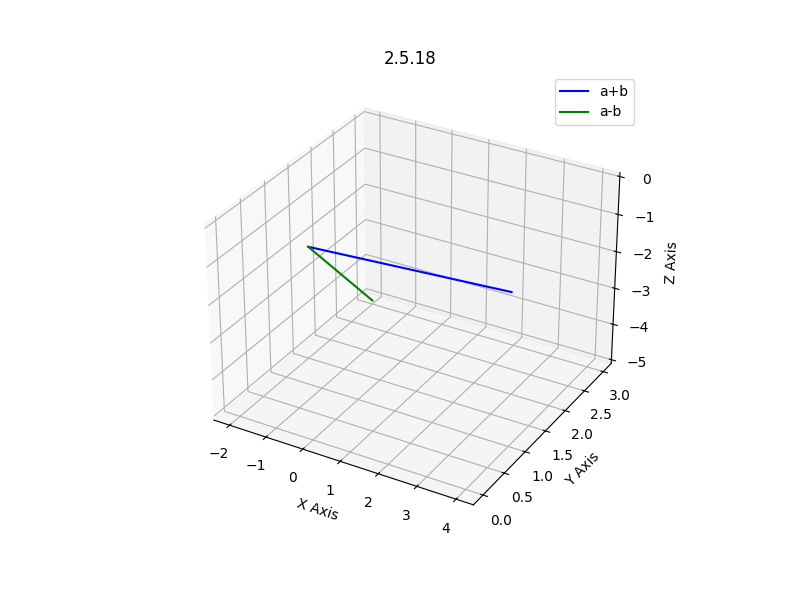
\includegraphics[width=0.8\columnwidth]{../figs/plot.png}
    \caption*{}
    \label{fig:plot}
\end{figure}
\end{frame}

\section{C Code}
\begin{frame}[fragile]{C code for generating points on line}
\begin{lstlisting}[language=C]
 void point_gen(const double* P1, const double* P2, double t, double* result_point) {
    result_point[0] = P1[0] + t * (P2[0] - P1[0]);
    result_point[1] = P1[1] + t * (P2[1] - P1[1]);
    result_point[2] = P1[2] + t * (P2[2] - P1[2]);
}
\end{lstlisting}
\end{frame}
\begin{frame}[fragile]{C Code for vector operations}
 \begin{lstlisting}[language=C]
  void vec_sum(const double* vec1, const double* vec2, double* sum) {
    sum[0] = vec1[0] + vec2[0];
    sum[1] = vec1[1] + vec2[1];
    sum[2] = vec1[2] + vec2[2];
}
void vec_diff(const double* vec1, const double* vec2, double* diff) {
    diff[0] = vec1[0] - vec2[0];
    diff[1] = vec1[1] - vec2[1];
    diff[2] = vec1[2] - vec2[2];
}
 \end{lstlisting}
\end{frame}
\section{Python Code}
\subsection{Using shared objects}
\begin{frame}[fragile]{Python code for plotting using C}
\begin{lstlisting}[language=Python]
import ctypes
import numpy as np
import numpy.linalg as LA
import matplotlib.pyplot as plt
from mpl_toolkits.mplot3d import Axes3D

libline = ctypes.CDLL("./line.so")
libvec = ctypes.CDLL("./vector.so")

get_point = libline.point_gen
get_point.argtypes = [
    ctypes.POINTER(ctypes.c_double),  # P1
    ctypes.POINTER(ctypes.c_double),  # P2
    ctypes.c_double,  # t
    ctypes.POINTER(ctypes.c_double),  # result_point
]
get_point.restype = None
\end{lstlisting}
\end{frame}
\begin{frame}[fragile]
 \begin{lstlisting}[language=Python]
add = libvec.vec_sum
add.argtypes = [
    ctypes.POINTER(ctypes.c_double),  # vec1
    ctypes.POINTER(ctypes.c_double),  # vec2
    ctypes.POINTER(ctypes.c_double),  # sum
]
add.restype = None
diff = libvec.vec_diff
diff.argtypes = [
    ctypes.POINTER(ctypes.c_double),
    ctypes.POINTER(ctypes.c_double),
    ctypes.POINTER(ctypes.c_double)]
diff.restype = None
DoubleArray3 = ctypes.c_double * 3
o = DoubleArray3(0, 0, 0)
a = DoubleArray3(1, 2, -3)
b = DoubleArray3(3, -1, 2)
c = DoubleArray3()
d = DoubleArray3()
 \end{lstlisting}
\end{frame}
\begin{frame}[fragile]
 \begin{lstlisting}[language=Python]
add(a, b, c)
diff(a, b, d)
fig = plt.figure(figsize=(8, 6))
ax = fig.add_subplot(111, projection="3d")
t_values = np.linspace(0, 1, 100)
line_points_x, line_points_y, line_points_z = [], [], []
for t in t_values:
    result_arr = DoubleArray3()
    get_point(o, c, t, result_arr)
    line_points_x.append(result_arr[0])
    line_points_y.append(result_arr[1])
    line_points_z.append(result_arr[2])
ax.plot(
    line_points_x,
    line_points_y,
    line_points_z,
    color="blue",
    label="a+b",
)
 \end{lstlisting}
\end{frame}
\begin{frame}[fragile]
 \begin{lstlisting}[language=Python]
t_values = np.linspace(0, 1, 100)
line_points_x, line_points_y, line_points_z = [], [], []

for t in t_values:
    result_arr = DoubleArray3()

    get_point(o, d, t, result_arr)

    line_points_x.append(result_arr[0])
    line_points_y.append(result_arr[1])
    line_points_z.append(result_arr[2])

ax.plot(
    line_points_x,
    line_points_y,
    line_points_z,
    color="green",
    label="a-b",
)
 \end{lstlisting}
\end{frame}
\begin{frame}[fragile]
 \begin{lstlisting}[language=Python]
ax.set_xlabel("X Axis")
ax.set_ylabel("Y Axis")
ax.set_zlabel("Z Axis")
ax.set_title("2.5.18")
ax.legend()
ax.grid(True)

plt.savefig("../figs/plot.png")
plt.show()
 \end{lstlisting}
\end{frame}
\subsection{Plot}
\begin{frame}{Plot}
 \begin{figure}[H]
    \centering
    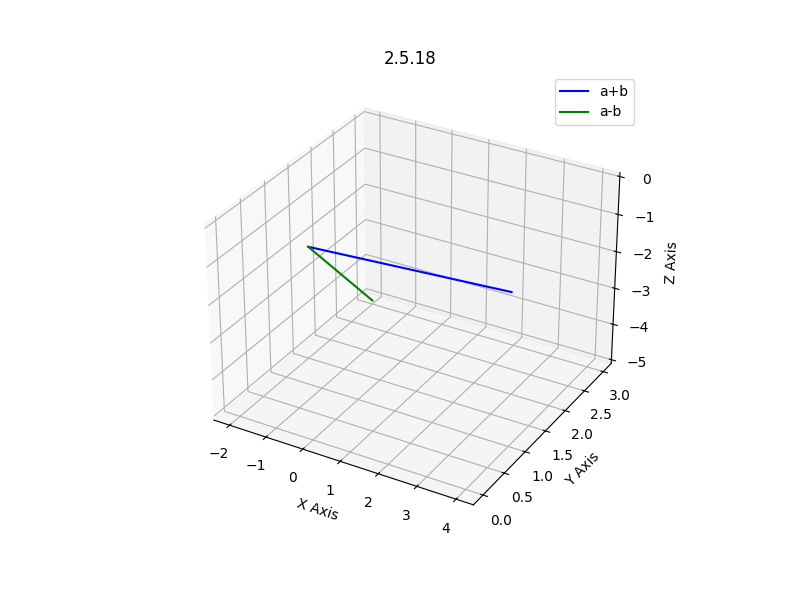
\includegraphics[width=0.8\columnwidth]{../figs/plot.png}
    \caption*{}
    \label{fig:plot}
\end{figure}
\end{frame}
\subsection{In pure Python}
\begin{frame}[fragile]{Pure Python code}
 \begin{lstlisting}[language=Python]
import numpy as np
import matplotlib.pyplot as plt
from mpl_toolkits.mplot3d import Axes3D

a = np.array([1, 2, -3]).T
b = np.array([3, -1, 2]).T

# Solving
c = a + b
d = a - b
result = (c.T) @ d
if result == 0:
    print("a+b and a-b are perpendicular")
else:
    print("a+b and a-b are not perpendicular")
 \end{lstlisting}
\end{frame}
\begin{frame}[fragile]{Pure Python code}
 \begin{lstlisting}[language=Python]
# Plotting
fig = plt.figure(figsize=(8, 8))
ax = fig.add_subplot(111, projection="3d")

ax.quiver(0, 0, 0, c[0], c[1], c[2], color="red", label="a+b")
ax.quiver(0, 0, 0, d[0], d[1], d[2], color="blue", label="a-b")

ax.set_xlabel("X-axis")
ax.set_ylabel("Y-axis")
ax.set_zlabel("Z-axis")
ax.set_title("2.5.18")
ax.set_xlim([-5, 5])
ax.set_ylim([-5, 5])
ax.set_zlim([-5, 5])
ax.legend()
ax.grid(True)
plt.savefig("../figs/python.png")
plt.show()
 \end{lstlisting}
\end{frame}
\subsection{Plot}
\begin{frame}{Plot}
 \begin{figure}[H]
    \centering
    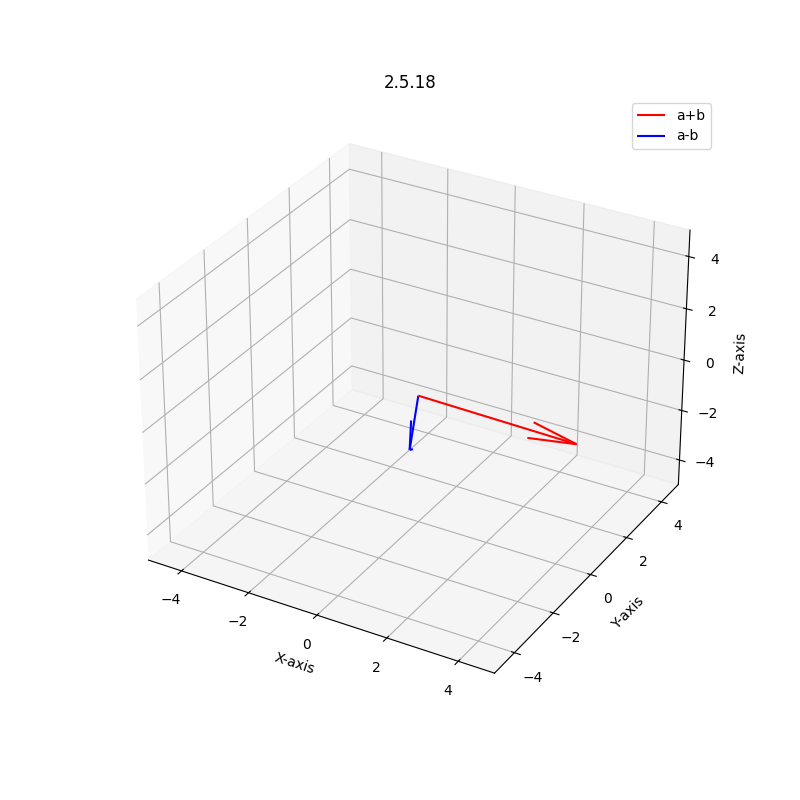
\includegraphics[width=0.75\columnwidth]{../figs/python.png}
    \caption*{}
    \label{fig:plot}
\end{figure}
\end{frame}
\end{document}
